
\section{link-analysis}\label{sec:graphs:link-analysis}
\Warning[TODO]{ title? Where? What? How? :) }

\begin{enumerate}
    \item Plot the whole function space (limited ofc)
    \item Scatter table with randomized large values
\end{enumerate}

\subsection{$\gamma$}

\FloatBarrier

\begin{figure}[h!]
  \centering
    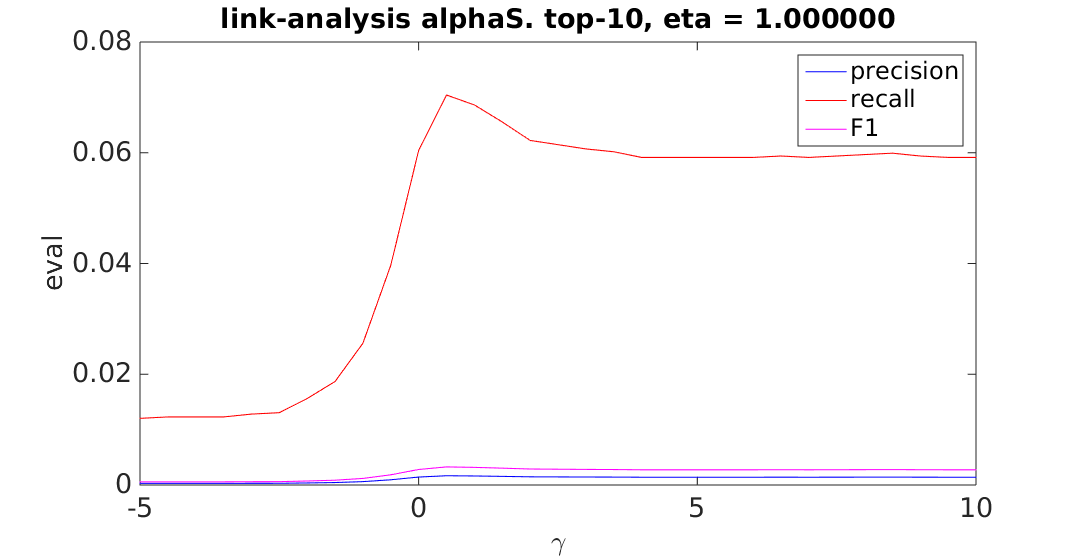
\includegraphics[width=0.9\textwidth]{fig/link_gamma/alphaS_link_gamma.png}
    \caption{\textit{alphaS}}
    \vspace{-10pt}
\end{figure}

\begin{figure}[h!]
  \centering
    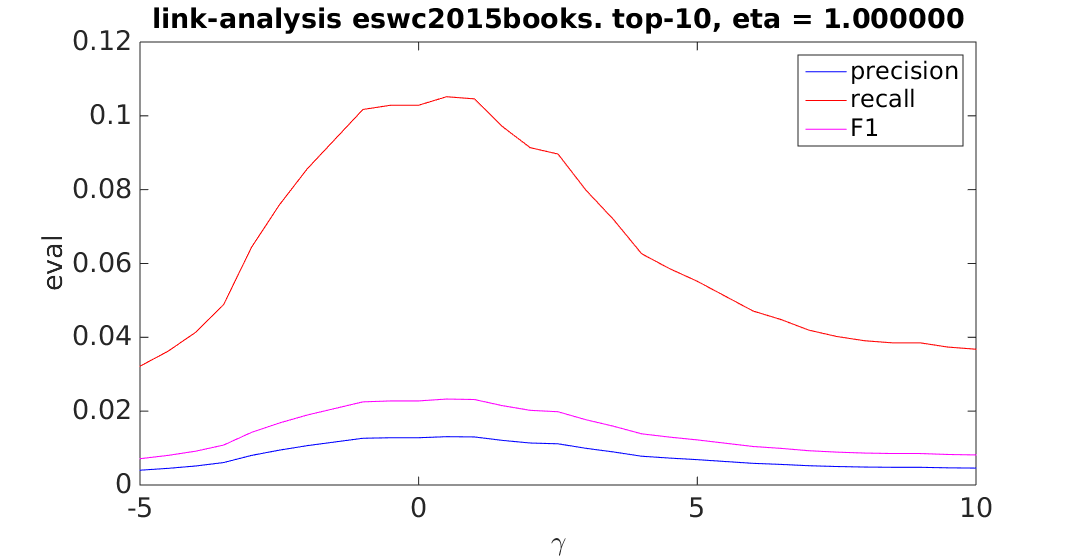
\includegraphics[width=0.9\textwidth]{fig/link_gamma/eswc2015books_link_gamma.png}
    \caption{\textit{eswc2015books}}
    \vspace{-10pt}
\end{figure}

\begin{figure}[h!]
  \centering
    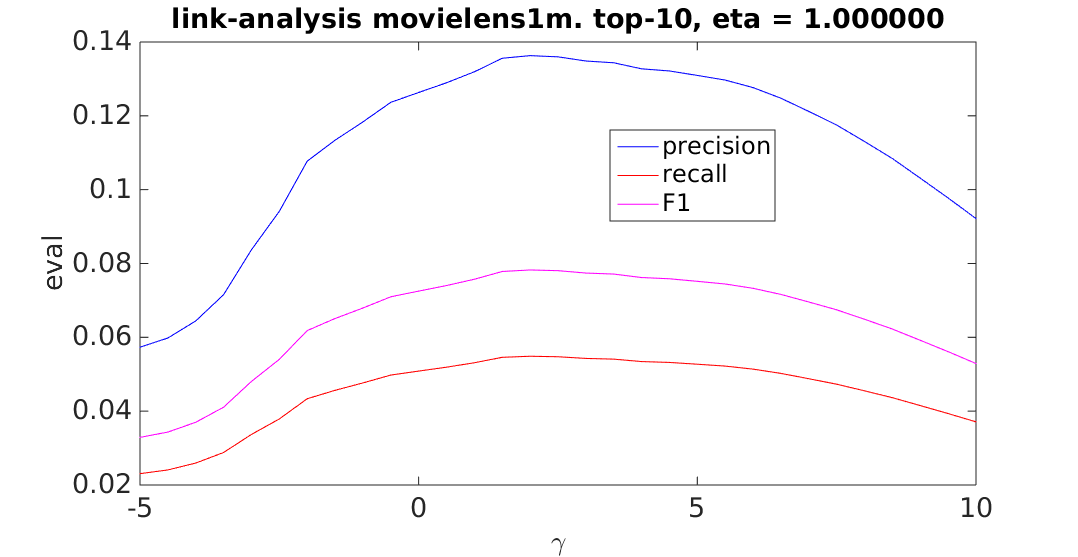
\includegraphics[width=0.9\textwidth]{fig/link_gamma/movielens_link_gamma.png}
    \caption{\textit{movielens1m}}
    \vspace{-10pt}
\end{figure}

\begin{figure}[h!]
  \centering
    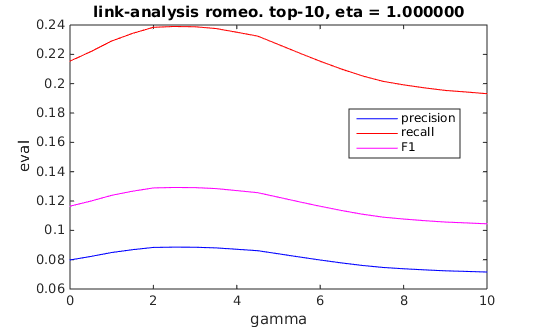
\includegraphics[width=0.9\textwidth]{fig/link_gamma/romeo_link_gamma.png}
    \caption{\textit{romeo}}
    \vspace{-10pt}
\end{figure}

\FloatBarrier


\newpage
\subsection{$\eta$}

\FloatBarrier

\begin{figure}[h!]
  \centering
    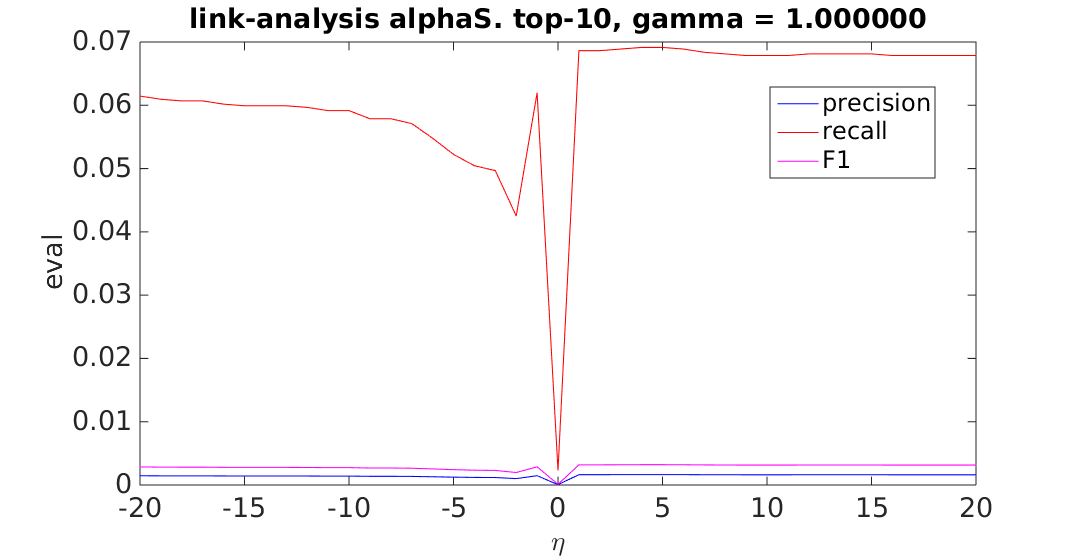
\includegraphics[width=0.9\textwidth]{fig/link_eta/alphaS_link_eta.png}
    \caption{\textit{alphaS}}
    \vspace{-10pt}
\end{figure}

\begin{figure}[h!]
  \centering
    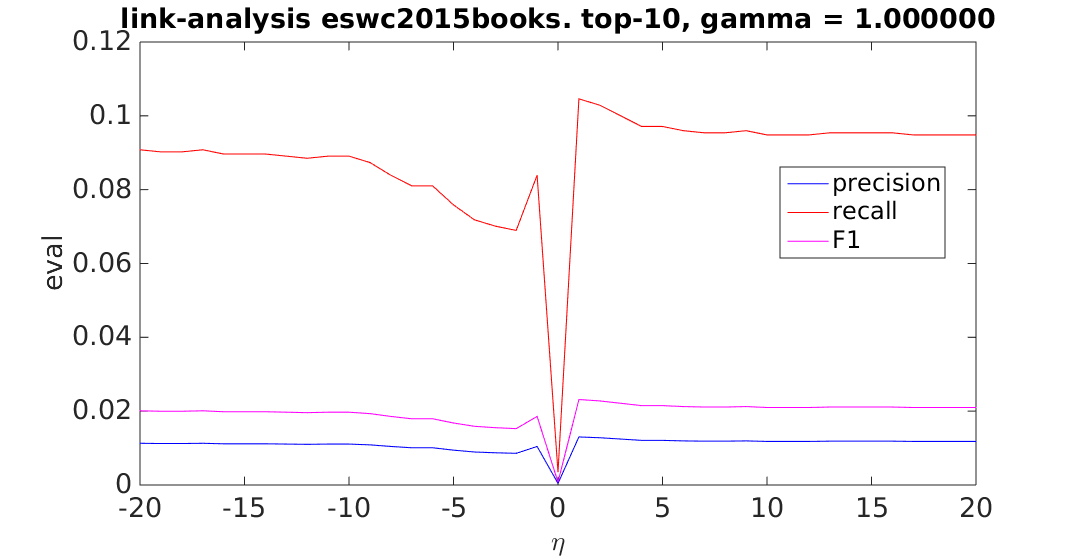
\includegraphics[width=0.9\textwidth]{fig/link_eta/eswc2015books_link_eta.png}
    \caption{\textit{eswc2015books}}
    \vspace{-10pt}
\end{figure}

\begin{figure}[h!]
  \centering
    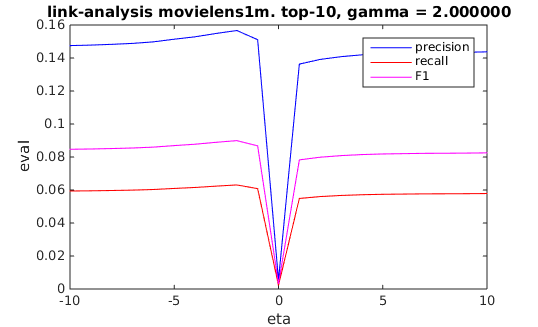
\includegraphics[width=0.9\textwidth]{fig/link_eta/movielens_link_eta.png}
    \caption{\textit{movielens1m}}
    \vspace{-10pt}
\end{figure}

\begin{figure}[h!]
  \centering
    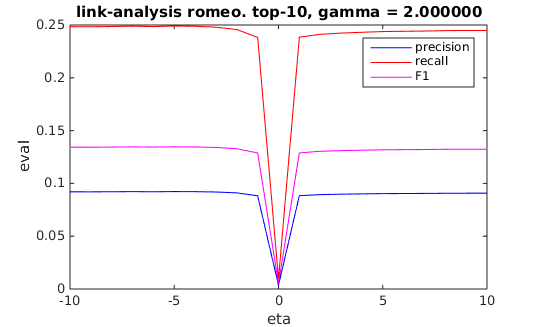
\includegraphics[width=0.9\textwidth]{fig/link_eta/romeo_link_eta.png}
    \caption{\textit{romeo}}
    \vspace{-10pt}
\end{figure}

\FloatBarrier

